\documentclass[11pt]{article}
\usepackage[paperwidth=254mm,paperheight=142.875mm,margin=12mm]{geometry}
\usepackage{amsmath,amssymb}
\usepackage{graphicx}
\usepackage{booktabs}
\usepackage{xcolor}
\usepackage{tikz}
\usepackage{listings}

\newcommand{\R}{\mathbb{R}}
\newcommand{\Var}{\operatorname{Var}}
\newcommand{\Cov}{\operatorname{Cov}}
\newcommand{\one}{\mathbf 1}

\newcommand{\slide}[1]{\clearpage\noindent{\Large\bfseries #1}\par\vspace{4pt}\hrule\vspace{10pt}}

\definecolor{ste}{RGB}{190,30,30}
\definecolor{rdg}{RGB}{30,80,190}

\lstset{language=Python, basicstyle=\ttfamily\footnotesize, columns=fullflexible, keepspaces=true,
  commentstyle=\color{black!55}, keywordstyle=\bfseries, showstringspaces=false, aboveskip=2pt, belowskip=2pt}

\setlength{\parindent}{0pt}

\begin{document}

% 1. TITLE
\clearpage
\vspace*{\fill}
\begin{center}
{\LARGE\bfseries Robust Training of Neural Networks\\[4pt] at Arbitrary Precision and Sparsity}\par\vspace{8pt}
{\large C.~Ye, G.~Chu, Y.~Liu, Y.~Zhang, L.~Lew, L.~Zhang, M.~Sandler, A.~Howard}\par
{\large Google DeepMind \quad\textbullet\quad ICLR 2026}\par\vspace{28pt}
{\large Presented by}\par\vspace{6pt}
{\Large Ayush Srivastava (2026AIB2015)\qquad Sarvesh Nikas (2026AIB2045)}
\end{center}
\vspace*{\fill}

% 2. SETUP
\slide{Quantization and the forward pass during training}

\textbf{Why.} A language model has billions of weights, each a 16- or 32-bit float: too big for a phone, slow, and costly in energy. Quantization stores each number with $k$ bits ($k=4,2,1$). Notation A$a$W$w$: $a$-bit activations, $w$-bit weights. At A1W1 a matrix multiply becomes XNOR and bit-counting.

\vspace{6pt}
\textbf{Training (QAT).} Keep the float block $x\in\R^N$ and update it by gradient descent, but run the forward pass on its quantized version, so the network learns to live with rounding. After training only the integers $q$ and one scale and offset per block are kept.
\[
x\ \xrightarrow{\ f\ }\ f(x)\ \xrightarrow{\ \operatorname{round}\ }\ q\ \xrightarrow{\ \text{dequantize}\ }\ \hat x\ \longrightarrow\ \text{rest of network}\ \longrightarrow\ L
\]
\begin{itemize}
\item $f(x)=\dfrac{x-b_f\one}{s_f}$ rescales $x$ onto the grid $\{0,\dots,2^k-1\}$, with $s_f=\dfrac{x_{\max}-x_{\min}}{2^k-1}$, $b_f=x_{\min}$ (affine; linear has $b_f=0$).
\item $q=\operatorname{round}\big(f(x)\big)=f(x)+\delta$: the stored integers, with rounding error $|\delta_i|\le\frac12$.
\item Standard dequantization: $\hat x=s_f\,q+b_f\one=x+s_f\,\delta$. This is what the next layer uses.
\end{itemize}

\textbf{Example} ($k=2$). $x=(0.9,\,-0.3,\,0.1,\,0.6)$: $s_f=0.4$, $b_f=-0.3$, $f(x)=(3,\,0,\,1,\,2.25)$, $q=(3,\,0,\,1,\,2)$, $\hat x=(0.9,\,-0.3,\,0.1,\,\mathbf{0.5})$.

% 3. PROBLEM
\slide{The problem: rounding has no gradient, and STE patches it blindly}

\begin{minipage}[t]{0.56\textwidth}
\textbf{Zero gradient.} By the chain rule the scalings cancel:
\[
\frac{\partial \hat x}{\partial x}=s_f\cdot\frac{\partial q}{\partial f(x)}\cdot\frac{1}{s_f}=\operatorname{round}'\big(f(x)\big)=0\ \text{ almost everywhere,}
\]
so $\nabla_xL=0$: $x$ and every earlier layer never update.

\vspace{6pt}
\textbf{Straight-Through Estimator} (Bengio et al., 2013). Round in the forward pass, pretend it is the identity in the backward pass:
\[
q=f(x)+\delta,\qquad \delta=\operatorname{stopgrad}\big(\operatorname{round}(f(x))-f(x)\big).
\]
\[
\text{forward: }\ \hat x=x+s_f\,\delta,\qquad\quad \text{backward: }\ \frac{\partial\hat x}{\partial x}=I^{\,*}.
\]

\textbf{The blind spot.} The forward pass shifts every entry by $s_f\delta_i$, but the backward pass is the same as with no quantization: $\delta$ never reaches the gradient (the paper's ``ghost of departed quantities''). Earlier layers get no signal about how rounding hurts the loss. Harmless at 8 bits; at 1--2 bits $s_f\delta$ is as large as the weights and training becomes unstable.
\end{minipage}\hfill
\begin{minipage}[t]{0.40\textwidth}\vspace{0pt}\centering
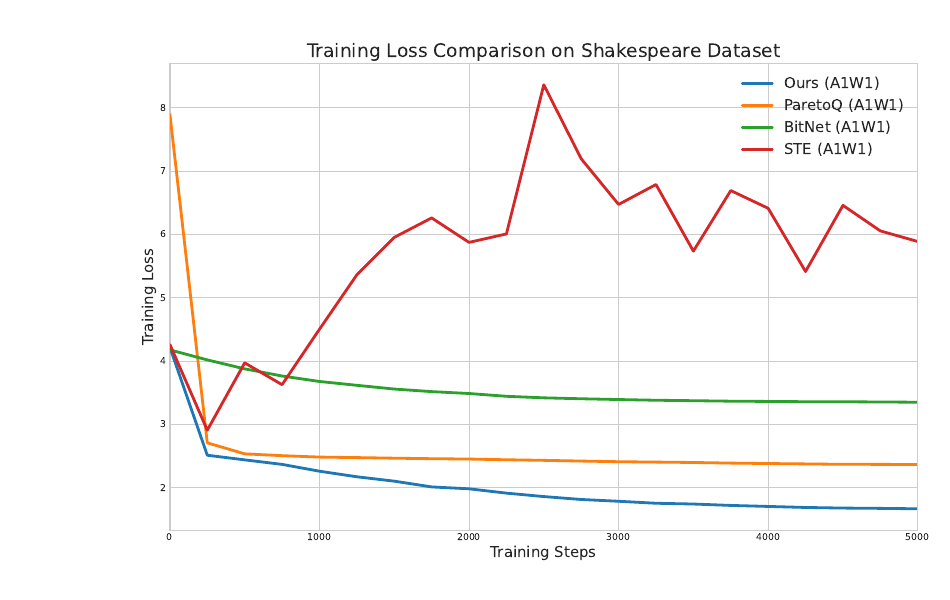
\includegraphics[width=\linewidth]{figs/fig1a_ste_divergence.png}\\[4pt]
\small Paper Fig.~1a: training loss at A1W1, small GPT on Shakespeare. STE (red) diverges; the paper's method (blue) converges.
\end{minipage}

\vfill
{\footnotesize $^*$Treating $s_f,b_f$ as constants; they depend on $x$ only through $x_{\min},x_{\max}$.}

% 4. MAIN IDEA
\slide{Main idea: dequantize by ridge regression}

\begin{minipage}[t]{0.56\textwidth}
Keep $f$ and round. Replace $\hat x=s_fq+b_f\one$ by the best affine fit of $x$ from $q$:
\[
\min_{s_g,\,b_g}\ \frac{1}{2N}\big\|s_g\,q+b_g\one-x\big\|^2+\frac{\lambda}{2}s_g^2
\quad\Longrightarrow\quad
g(q)=\underbrace{\frac{\Cov_{xq}}{\Var_q+\lambda}}_{s_g}\,(q-\bar q\one)+\bar x\one .
\]
\begin{itemize}
\item $s_g,b_g$ come from the block's statistics at every step: nothing to learn, nothing to tune.
\item Never worse: with $\lambda=0$, $g(q)$ is the orthogonal projection of $x$ onto $\operatorname{span}\{\one,q\}$, and $\hat x$ lies in that span, so $\|x-g(q)\|\le\|x-\hat x\|$.
\item Example of slide 2: $g(q)=(0.935,\,-0.285,\,0.122,\,0.528)$; squared error $0.010\to0.007$.
\item $\lambda$ gives stability ($\Var_q=0$ would give $0/0$; $\lambda=0$ produces NaN) and denoising ($\lambda\to\infty$ gives $g\to\bar x\one$). One value, $\lambda=0.01$, is used everywhere.
\item Same form and cost as a LayerNorm: $\Var_q+\lambda$ plays the role of $\sigma^2+\epsilon$.
\end{itemize}
\end{minipage}\hfill
\begin{minipage}[t]{0.40\textwidth}\vspace{0pt}\centering
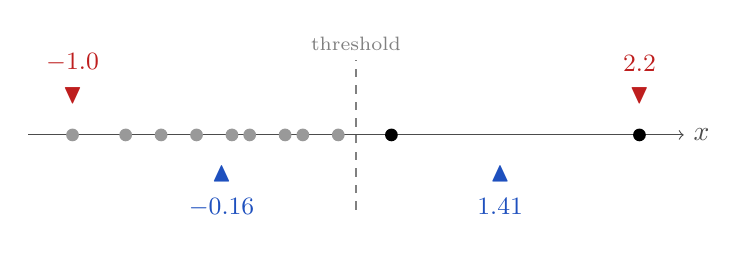
\begin{tikzpicture}[x=2.25cm,y=1cm]
\draw[->,black!70] (-1.25,0) -- (2.45,0) node[right] {$x$};
\draw[dashed,black!50] (0.6,-0.95) -- (0.6,0.95);
\foreach \v in {-1.0,-0.7,-0.5,-0.3,-0.1,0.0,0.2,0.3,0.5} \fill[black!40] (\v,0) circle (2.3pt);
\foreach \v in {0.8,2.2} \fill[black] (\v,0) circle (2.3pt);
\foreach \v/\t in {-1.0/{-1.0},2.2/{2.2}} {
  \node[ste] at (\v,0.5) {$\blacktriangledown$};
  \node[ste,above] at (\v,0.68) {\small $\t$};}
\foreach \v/\t in {-0.159/{-0.16},1.414/{1.41}} {
  \node[rdg] at (\v,-0.5) {$\blacktriangle$};
  \node[rdg,below] at (\v,-0.68) {\small $\t$};}
\node[black!50,above] at (0.6,0.95) {\scriptsize threshold};
\end{tikzpicture}\\[6pt]
\small 1 bit, 11 weights with one outlier. Both methods give the same $q$ (grey $\to0$, black $\to1$). STE ({\color{ste}$\blacktriangledown$}) maps $q$ back to $x_{\min},x_{\max}$; ridge ({\color{rdg}$\blacktriangle$}) to roughly the two group means. Squared error $9.98\to2.93$.
\end{minipage}

% 5. WHY IT WORKS
\slide{Why it works: what the backward pass sees}

\textbf{Honest starting point.} Ridge still sends the gradient straight through round ($\delta$ is detached, exactly as in STE). What changes is the function around round.

\vspace{4pt}
\textbf{A true gradient now exists.} Inside a rounding cell $q$ is constant, yet $g$ still depends on $x$ through $\bar x$ and $\Cov_{xq}$. So the deployed map $x\mapsto g\big(\operatorname{round}(f(x)),x\big)$ has a true Jacobian $P$ (the projection onto $\operatorname{span}\{\one,q\}$): it moves the levels. For STE the true Jacobian is $0$.

\vspace{4pt}
\textbf{Jacobian used in training} (our derivation; it matches autograd to machine precision$^*$):
\[
J_{\text{STE}}=\underbrace{0}_{\text{exact}}+\underbrace{I}_{\text{surrogate}},
\qquad\qquad
J_{\text{ridge}}=\underbrace{P}_{\text{exact}}+\underbrace{\rho\,(I-P)}_{\text{surrogate}}+\underbrace{c\,u\,r^{\top}}_{\text{error term}},
\]
\[
u=q-\bar q\one,\quad r=x-g(q),\quad \rho=\frac{s_g}{s_f},\quad c=\frac{1}{s_fN(\Var_q+\lambda)},\quad P=\frac{\one\one^{\top}}{N}+\frac{uu^{\top}}{N(\Var_q+\lambda)}.
\]
\begin{enumerate}
\item \textbf{Exact where possible.} The surrogate is used only for moving entries across rounding boundaries.
\item \textbf{The surrogate is damped.} $\rho=s_g/s_f$ was $0.29,\ 0.87,\ 0.99$ at $k=1,2,4$ (Gaussian block, $N=64$). The coarser the rounding, the less the guess is trusted; at 4 bits ridge $\approx$ STE.
\item \textbf{The error itself is in the gradient.} $\nabla_xL$ gains the term $c\,r\,(u^{\top}\nabla_gL)$, where $u^{\top}\nabla_gL=\partial L/\partial s_g$: when the loss wants a different scale, $x$ moves along its own error $r$. The term vanishes when $r=0$.
\end{enumerate}

\vfill
{\footnotesize $^*$For all entries except the block's min and max. The paper's own version (App.~A.4): $\partial g/\partial q=s_g I+q\,(\nabla_q s_g)^{\top}$ depends on $\delta$ through $q$.}

% 6. EXTENSIONS
\slide{Extensions: sparsity, and a fast affine matrix multiply}

\begin{minipage}[t]{0.44\textwidth}
\textbf{Sparsity is quantization to zero.}
\begin{itemize}
\item Prune first: $\delta_S=\operatorname{threshold}(x)-x$ (e.g.\ keep the 2 largest of every 4), $x_S=x+\delta_S$.
\item Then quantize: $q=f(x_S)+\delta_Q$.
\item $g(q)$ is fitted to the dense float $x$, so both passes see the total error $\delta_S+\delta_Q$.
\item 1-bit weights with 1:4 sparsity: (1 value bit $+$ 2-bit position)$/4=0.75$ bits per weight, i.e.\ below 1 bit.
\item Gemma3 1B at A4W1: 2:4 sparsity halves the compute cost and raises accuracy $0.4056\to0.4080$.
\end{itemize}
\end{minipage}\hfill
\begin{minipage}[t]{0.52\textwidth}
\textbf{Theorem 1 (affine matmul shortcut).} Dequantize the rows of $X\in\R^{M\times n}$ and the columns of $W\in\R^{n\times P}$ with $g$:
\[
\tilde X=(s_X\one^{\top})\odot(Q_X-\bar q_X\one^{\top})+\bar x\one^{\top},\qquad
\tilde W=(Q_W-\one\bar q_W^{\top})\odot(\one s_W^{\top})+\one\bar w^{\top}.
\]
Then
\[
\boxed{\ \tilde X\tilde W=(s_Xs_W^{\top})\odot\big(Q_XQ_W-n\,\bar q_X\bar q_W^{\top}\big)+n\,\bar x\,\bar w^{\top}\ }
\]
\textbf{Proof.} Centred rows and columns sum to zero, so both cross terms vanish, and $\one^{\top}\one=n$. Expanding the centred integer product gives $Q_XQ_W-n\,\bar q_X\bar q_W^{\top}$. $\square$

\vspace{4pt}
\textbf{Cost.} One integer matmul $O(MnP)$, two rank-1 terms $O(MP)$, statistics $O(Mn+nP)$: about the cost of linear quantization. This makes affine quantization affordable. We checked the identity numerically (error $3\times10^{-14}$).
\end{minipage}

% 7. PAPER RESULTS
\slide{Results from the paper}

\begin{minipage}[t]{0.42\textwidth}\vspace{0pt}
\centering
\begin{tabular}{lcc}
\toprule
Gemma3 1B, C4 accuracy & STE & ridge \\
\midrule
A4W4, affine, SCQ128 & 0.4254 & 0.4274 \\
A2W2, affine, SCQ128 & 0.3794 & 0.4027 \\
A1.5W1.5, linear, channel & NaN & 0.3297 \\
A1W1, linear, SCQ128 & 0.3399 & 0.3547 \\
A1W1, affine, SCQ128 & 0.3397 & 0.3751 \\
\bottomrule
\end{tabular}\\[6pt]
\raggedright\small SCQ128: one scale and offset per block of 128. The gap grows as bits fall. Affine gains nothing under STE ($0.3399\to0.3397$) but $+0.020$ under ridge.
\end{minipage}\hfill
\begin{minipage}[t]{0.54\textwidth}\vspace{0pt}
\begin{itemize}
\item \textbf{Stability.} nanoGPT on Shakespeare at A1W1: STE and BitNet diverge or stall; ridge converges (slide 3). This also holds with linear quantization for both: STE ends above 5.0 validation loss, ridge at about 2.1. On GPT-2 124M (OpenWebText), STE and BitNet are unstable or reach NaN.
\item \textbf{Storage frontier.} Best accuracy per weight bit comes from asymmetric A4W1, not A2W2: keep activations precise, compress static weights.
\item \textbf{Bigger and fewer bits wins.} Gemma3 4B at A4W1 with 2:4 sparsity (650 MB) reaches 0.4517, above Gemma3 1B in BF16 (1400 MB, 0.4494).
\item \textbf{Beyond LLMs, no tuning.} ResNet-50 on ImageNet: A4W4 76.45\% vs.\ float 76.41\%. WMT EN-DE: A4W4 29.71 vs.\ float 29.49 BLEU.
\end{itemize}
\end{minipage}

% 8. OUR IMPLEMENTATION
\slide{Our implementation: a toy reproduction}

\begin{minipage}[t]{0.50\textwidth}\vspace{0pt}
\textbf{Setup.} Char-level GPT (4 blocks, 0.82M parameters) on Tiny Shakespeare, 3000 steps, AdamW, one seed. All linear layers in the blocks at A$k$W$k$, affine, per row. Runs differ only in the dequantizer.

\vspace{4pt}
\textbf{Core code} (\texttt{quant.py}, condensed):
\begin{lstlisting}
def quantize(x, k):             # q = f(x) + stopgrad(delta)
    lo = x.amin(-1, keepdim=True)
    hi = x.amax(-1, keepdim=True)
    s_f = (hi - lo + 1e-8) / (2**k - 1)
    f_x = (x - lo) / s_f
    delta = (torch.round(f_x) - f_x).detach()
    return f_x + delta, s_f, lo

def x_hat(q, s_f, lo):          # STE: undo the rescale
    return s_f * q + lo

def g(q, x, lam=1e-2):          # ridge fit of x from q
    m = lambda t: t.mean(-1, keepdim=True)
    qc, xc = q - m(q), x - m(x)
    s_g = m(xc * qc) / (m(qc * qc) + lam)
    return s_g * qc + m(x)
\end{lstlisting}
\end{minipage}\hfill
\begin{minipage}[t]{0.47\textwidth}\vspace{0pt}
\centering
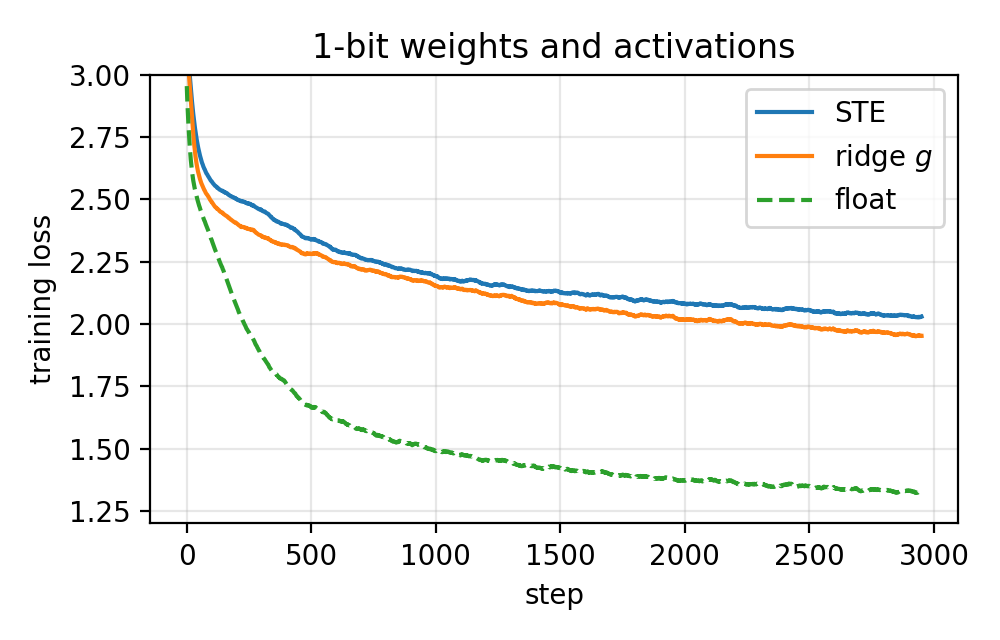
\includegraphics[height=40mm]{implementation/plots/loss_k1.png}
\hspace{2mm}
\small
\begin{tabular}[b]{ccc}
\toprule
bits & STE & ridge \\
\midrule
1 & 2.123 & 2.071 \\
2 & 1.812 & 1.790 \\
4 & 1.592 & 1.597 \\
\midrule
float & \multicolumn{2}{c}{1.586} \\
\bottomrule
\end{tabular}\\[2pt]
\raggedright
Final validation loss (right); training loss at A1W1 (left).
\begin{itemize}
\item Ridge is better at 1--2 bits and ties at 4 bits, as $\rho\to1$ predicts.
\item STE did not diverge at this scale (the paper used 11M parameters and 5000 steps).
\item Gradient check: same $q$, $\delta$ changed by up to 0.106. The gradient reaching $x$ changes by 0.0000 under STE and by up to 0.0144 under ridge.
\item Size at 1 bit: 3.27 MB $\to$ 256 kB ($12.7\times$). 47\% of that stays float: embeddings, output layer, LayerNorms.
\end{itemize}
\end{minipage}

% 9. PROS AND CONS
\slide{Advantages and disadvantages}

\begin{minipage}[t]{0.47\textwidth}
\textbf{Advantages}
\begin{itemize}
\item \textbf{Drop-in.} It replaces one function (about five lines). No learned quantizer parameters; one $\lambda=0.01$ everywhere; same hyperparameters as the BF16 baseline.
\item \textbf{Stable where STE fails.} A1W1, A1.5W1.5 and sub-1-bit train; the gain grows as bits fall.
\item \textbf{Better forward pass.} Reconstruction is never worse than standard dequantization ($\lambda=0$), at the cost of a LayerNorm.
\item \textbf{Affine pays off}, and Theorem 1 makes it cheap.
\item \textbf{One framework} for quantization and sparsity, with storage and energy trade-off curves for real LLMs.
\end{itemize}
\end{minipage}\hfill
\begin{minipage}[t]{0.49\textwidth}
\textbf{Disadvantages}
\begin{itemize}
\item \textbf{Still a surrogate through round.} ``Without gradient estimation'' is overstated; the exact part has rank 2 per block.
\item \textbf{Little gain at 4 bits} ($+0.002$), where most deployment happens today.
\item \textbf{Not free at inference.} $s_g,b_g$ per block of 128 add 0.125--0.25 bits per weight (8- or 16-bit values); activations need float $\bar x$ and $\Cov_{xq}$ at run time.
\item \textbf{Efficiency is estimated, not measured.} Energy $=$ sparsity $\times$ A-bits $\times$ W-bits $\times$ ops ignores data movement. All runs use simulated (fake) quantization; no speed is reported.
\item \textbf{Thin evidence.} Single runs, no error bars. $\lambda=0\to$ NaN is a $0/0$ in the forward pass, not proof of the gradient path. Small errors: the linear closed form misses a factor $N$ on $\lambda$, and the text after Eq.~6 has a typo.
\end{itemize}
\end{minipage}

% 10. OPINION
\slide{Our opinion and takeaway}

\textbf{The real contribution.} It is not ``no gradient estimation'': the guess through round is still there. The contribution is to change what surrounds the guess. A least-squares dequantizer gives an output closer to $x$ and a Jacobian that is exact on the levels, damps the guess, and carries the error $r$. It is simple, cheap and principled; we would use it for 1--2-bit training.

\vspace{6pt}
\textbf{Convincing.} The ablation is controlled: same surrogate, only $g$ changes, gains in every setting, and the gap grows as bits fall. The linear-vs-linear run rules out ``it is just affine''. Our $\rho$ analysis predicts the same pattern.

\vspace{6pt}
\textbf{Less convincing.}
\begin{itemize}
\item ``For the first time'': LSQ (Esser et al., 2019) already puts $\delta$ into the gradient of a learned step size, $\partial\hat x/\partial s=\operatorname{round}(x/s)-x/s=\delta$. Ridge fits scale and offset in closed form instead of learning them.
\item Theorem 1 is the mean-centring identity. It holds for any affine dequantizer, with that dequantizer's output mean in place of $\bar x$; we checked this numerically.
\item ``Theoretically grounded'' but there is no convergence result; the support is empirical.
\end{itemize}

\textbf{Next steps for us.} A $\lambda$ sweep and linear vs.\ affine in our toy; several seeds; the paper's 11M model to see STE diverge; real integer kernels for wall-clock time.

\vfill
\fbox{\parbox{\dimexpr\textwidth-2\fboxsep-2\fboxrule}{\centering\large
\textbf{Takeaway:} do not ignore the quantization error; fit it. A ridge-regression dequantizer makes the forward pass less noisy and the backward pass error-aware, and that is enough to make 1-bit training stable.}}

\end{document}
